\section{Estimation of backgrounds}
\label{sec:backgrounds}

\subsection{Multijets background}
\label{sec:qcd_background}

The signal region is defined in a manner to suppress the expected
contribution from multijet production to the percent level with
respect to the total expected background counts from other SM
processes for all event categories, defined in terms of \njet and \nb,
and all bins, defined in \scalht and \HTmiss. This is achieved
primarily through the application of very tight requirements on the
variables \alphat and \dphi, as described in
Section~\ref{sec:signal_region}, as well as the requirement $\mhtmet <
1.25$. In this section, we discuss these requirements further, and the
estimate of the suppression of the multijet background.

%The contamination from multijet events in the signal region is
%estimated using a multijet-enriched data sideband to the signal
%region, defined by the (inverted) requirement $\mhtmet > 1.25$. The
%observed counts in data are categorised according to \njet and \scalht
%and are corrected to account for contamination from vector boson and
%\ttbar production, and residual contributions from other SM processes,
%which are estimated using the \mj control region with the method
%described in Section~\ref{sec:ewk_background}. 
%The corrected data counts $\mathcal{N}^\text{data}(\njet, \scalht)$
%are used to estimate the multijet background in the signal region
%$\mathcal{P}(\njet, \scalht)$ through multiplication with the ratio
%$\mathcal{R}^\text{QCD}(\njet, \scalht)$ of multijet events that
%satisfy the requirement $\mhtmet < 1.25$ to those that fail, which is
%determined independently for events categorised according to \njet and
%\scalht from simulation. 
%Finally, the differential distribution of $\mathcal{P}(\njet,
%\scalht)$ as a function of \nb and \HTmiss is described by the
%multiplier term $\mathcal{K}_{\njet, \scalht}(\nb, \HTmiss)$, which is
%assumed to exhibit the same distribution as the non-multijet
%backgrounds, as determined from simulation.

The contamination from multijet events in the signal region is
estimated using a multijet-enriched data sideband to the signal
region, defined by the (inverted) requirement $\mhtmet > 1.25$. The
observed counts in data, categorised according to \njet and \scalht,
are corrected to account for contamination from non-multijet SM
processes, and the corrected counts $\mathcal{N}^\text{data}(\njet,
\scalht)$ are assumed to arise solely from QCD multijet
production. The non-multijet processes, which comprise vector boson
and \ttbar production, and residual contributions from other SM
processes, are estimated using the \mj control region using the method
described in Section~\ref{sec:ewk_background}. Independent ratios
$\mathcal{R}^\text{QCD}(\njet, \scalht)$ of multijet events that
satisfy the requirement $\mhtmet < 1.25$ to those that fail, where the
events are categorised according to \njet and \scalht, are determined
from simulation. The product of a ratio $\mathcal{R}^\text{QCD}(\njet,
\scalht)$ and a corrected data count $\mathcal{N}^\text{data}(\njet,
\scalht)$ provides the estimate of the multijet background
$\mathcal{P}(\njet, \scalht)$. Each estimate is assumed to distribute
identically to the non-multijet backgrounds as a function of \nb and
\HTmiss. This final assumption, implemented by the multiplier term
$\mathcal{K}_{\njet, \scalht}(\nb, \HTmiss)$, is based on studies in
simulation and is a valid approximation given the magnitude of the
uncertainties in the ratios $\mathcal{R}^\text{QCD}(\njet, \scalht)$,
described below. 
%assumed in the method to estimate this residual background
%contribution, described below.
%and is a valid approximation given the relatively low level of
%contamination and the magnitude of the uncertainty in the method,
%described below.
Assuming $i$, $j$, $k$, and $l$ are the bin indices for, respectively,
\njet, \scalht, \nb, and \HTmiss:

\begin{equation}
  \label{eq:qcd}
  \mathcal{P}( i, j, k, l ) =
  \mathcal{N}^\text{data}( i, j )\;
  \mathcal{R}^\text{QCD}( i, j )\;
  \mathcal{K}_{i,j}( k, l ).
\end{equation}

The use of simulation to determine $\mathcal{R}^\text{QCD}(\njet,
\scalht)$ is validated using a multijet-enriched data sideband defined
by $\bdphi < 0.5$.
%and an \alphat requirement identical to that used for the signal
%region, which is dependent on the value \scalht, as summarised in
%Table~\ref{}. 
The ratio $\mathcal{R}^\text{data}(\njet, \scalht)$ is constructed
from data counts, corrected to account for contributions from
non-multijet processes, and compared with
$\mathcal{R}^\text{QCD}(\njet, \scalht)$, determined from simulation,
through the double ratio
$\mathcal{R}^\text{data}/\mathcal{R}^\text{QCD}$, as shown in
Fig.~\ref{fig:qcd}. The double ratios are observed to be close to, or
statistically compatible with, unity across the full phase space of
the signal region, including the bins at high \scalht, which exhibit
the highest statistical precision. An uncertainty of 100\% in
$\mathcal{R}^\text{QCD}$ is assumed to adequately cover the observed
level of agreement for the full signal region phase space, as well as
any limitations in the assumptions on the distribution of multijet
events as a function of \nb and \HTmiss for all regions defined in
terms of \njet and \scalht.

\begin{figure}[!t]
  \begin{center}
%    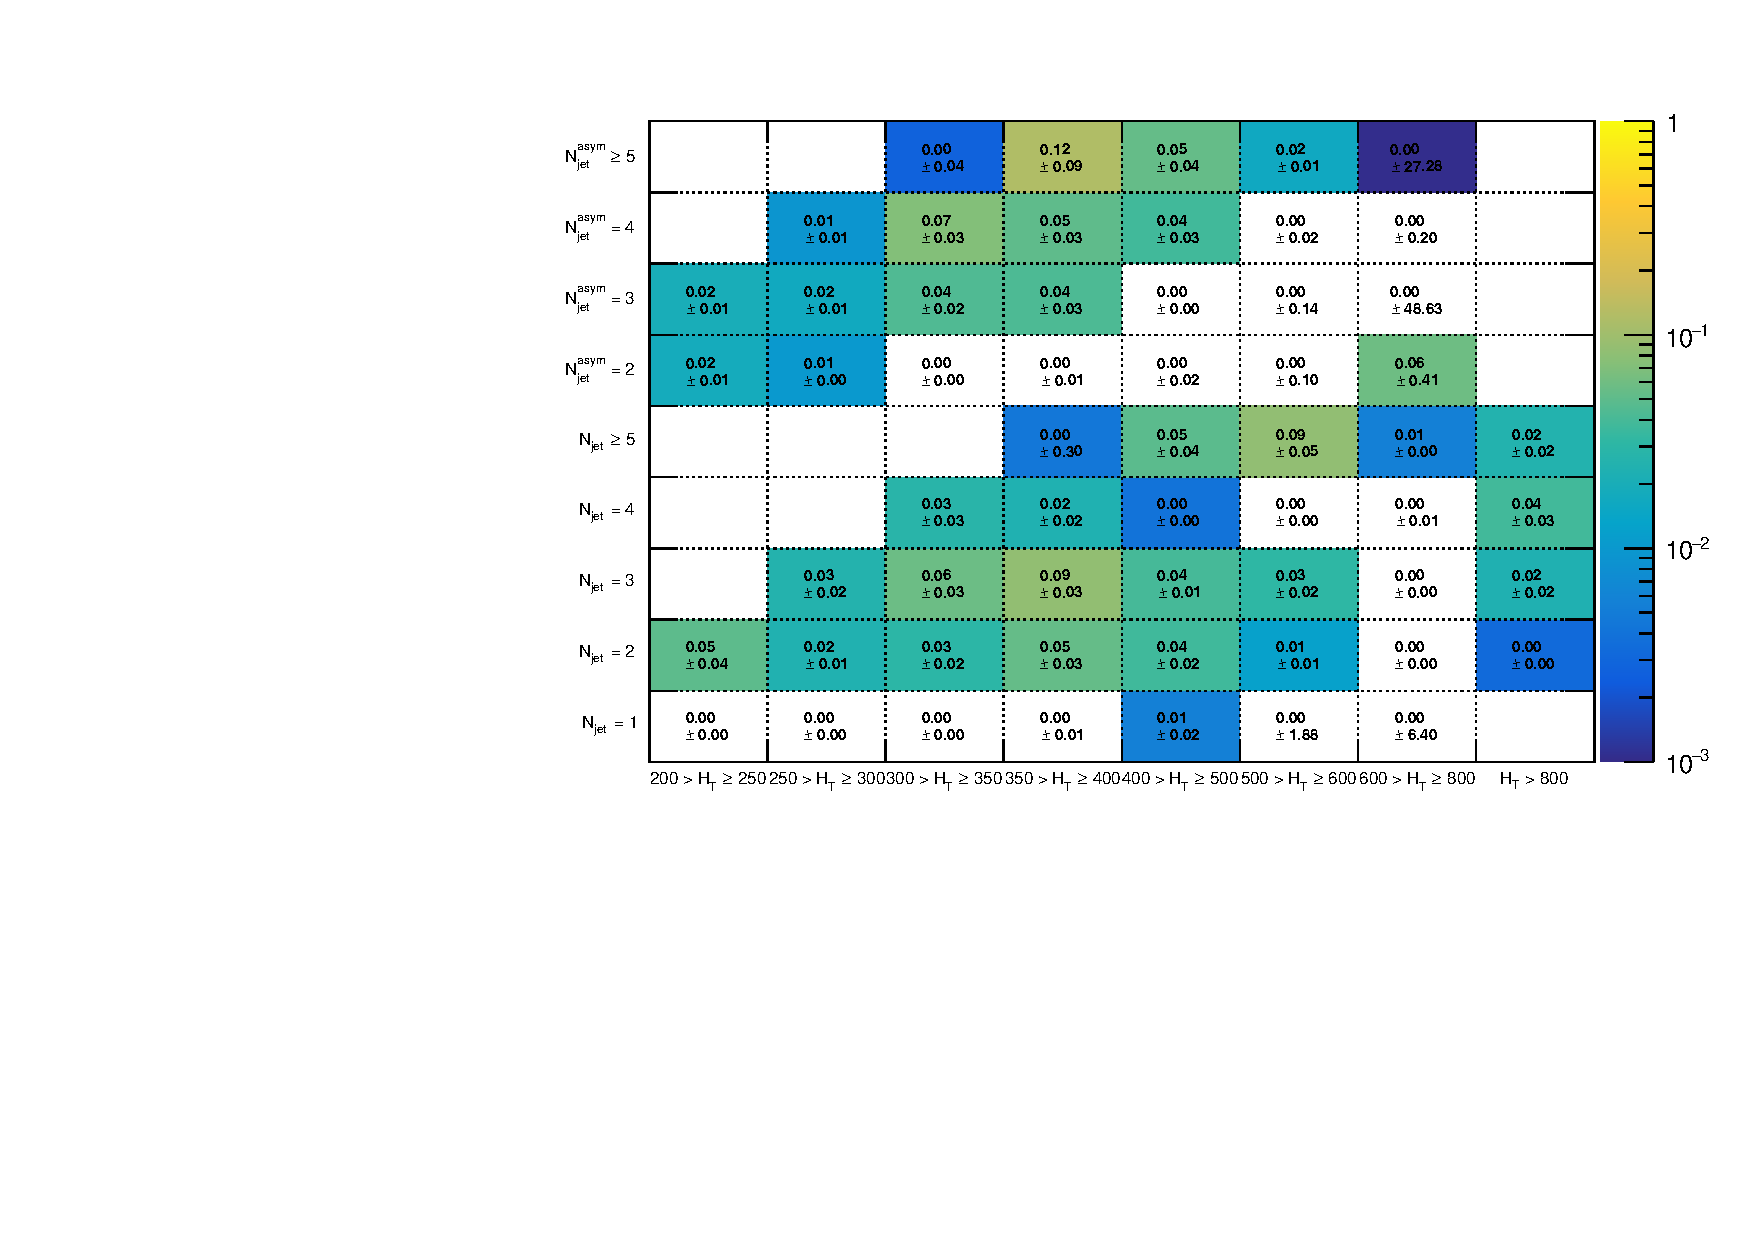
\includegraphics[width=0.49\textwidth]{figures/qcd/v0/qcd_pred} \,
    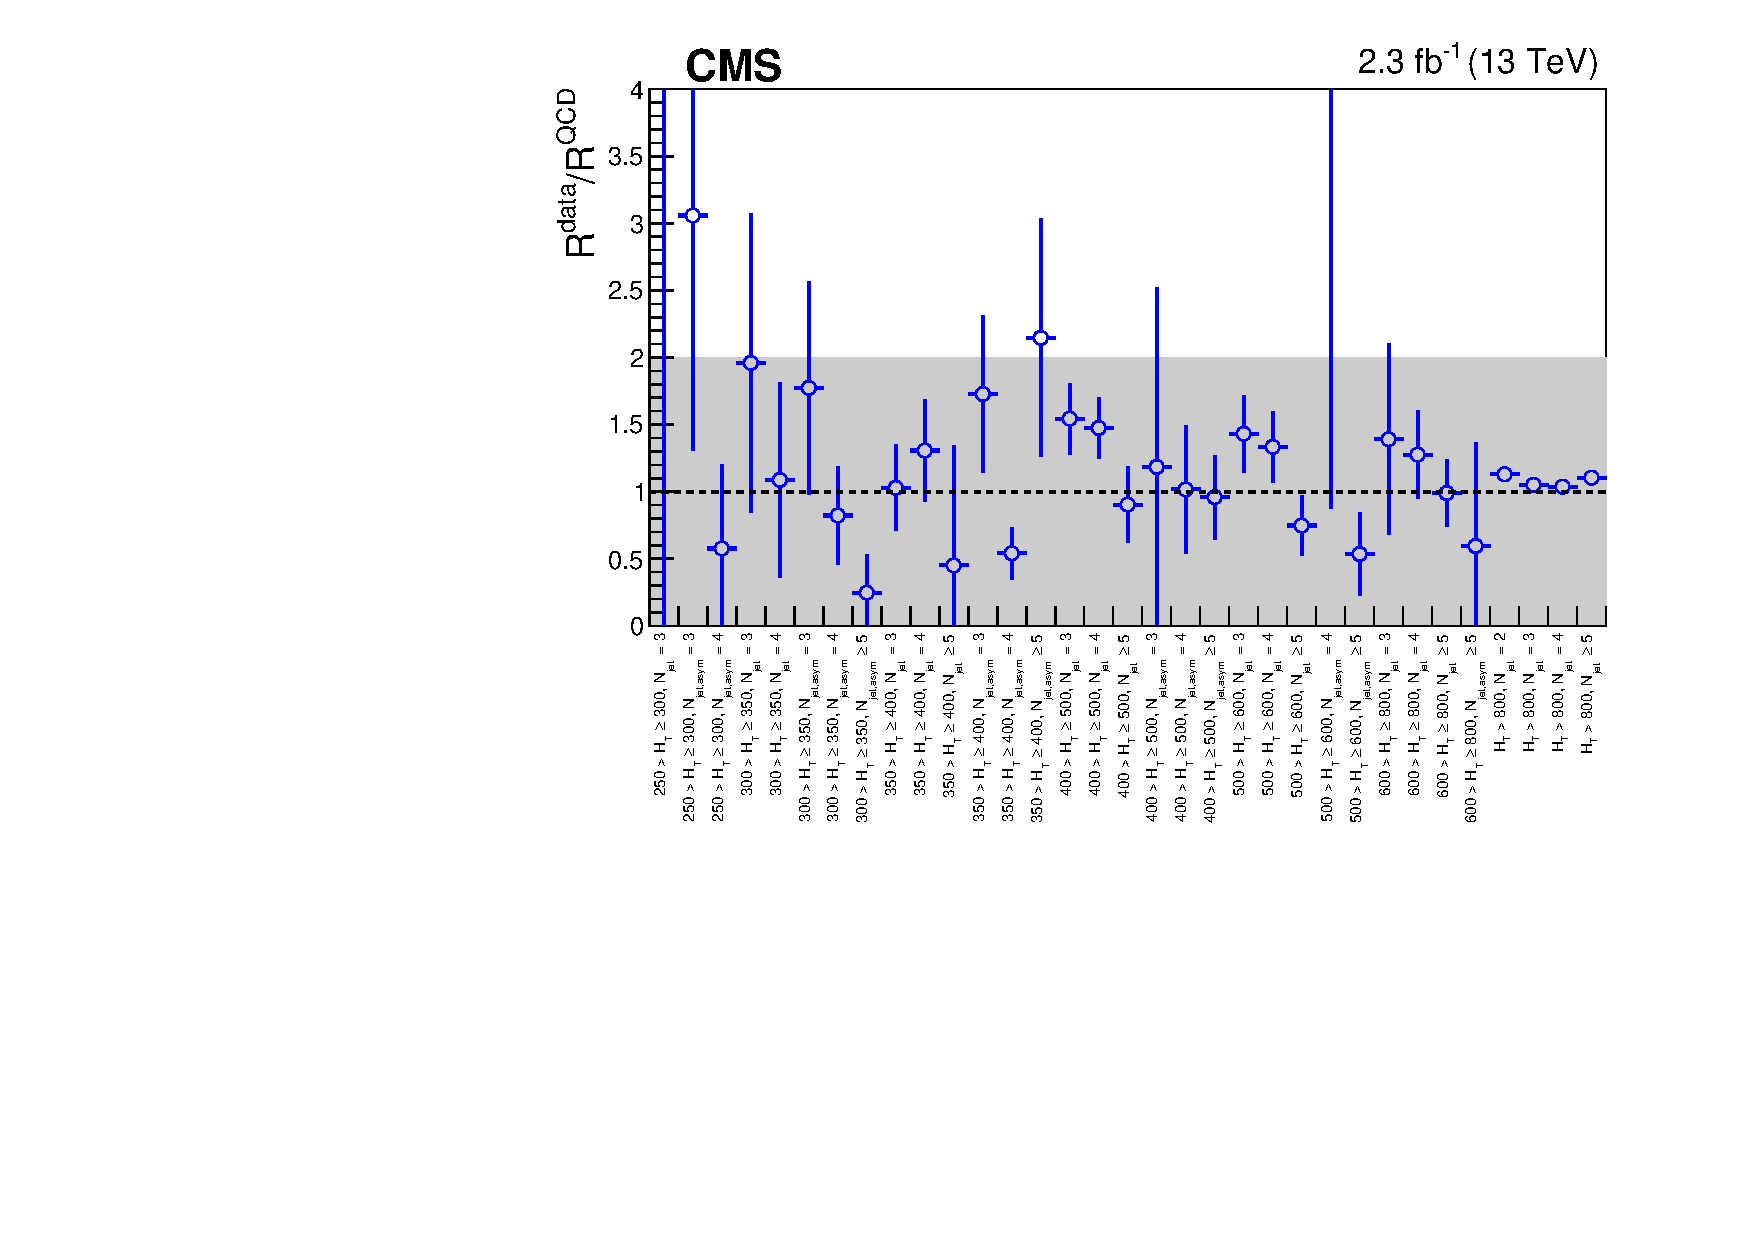
\includegraphics[width=0.7\textwidth]{figures/qcd/v1/DoubleRatioQCD_noEmpty} \\
  \end{center}
  \caption{Validation of the ratio $\mathcal{R}^\text{QCD}$ determined
    from simulation in bins of \njet and \scalht by comparing with an
    equivalent ratio $\mathcal{R}^\text{data}$ constructed from data 
    in a multijet-enriched sideband to the signal region. A value of
    unity is expected for the double ratio $\mathcal{R}^\text{data} /
    \mathcal{R}^\text{QCD}$, and the grey shaded band represents the
    assumed systematic uncertainty of 100\% in
    $\mathcal{R}^\text{QCD}$. 
  }
  \label{fig:qcd} 
\end{figure}

%Finally, data control variables, such as $\bdphimod$, are inspected
%for localised populations in $(\eta,\phi)$-space to provide confidence
%that any multijet contamination due to instrumental effects is
%negligible.
